
La dependencia de los combustibles fósiles traería consigo problemas como la inseguridad energética y el incremento de la temperatura global a causa del aumento de los gases de efecto invernadero. Las sociedades que concentran la producción de los combustibles fósiles podrían controlar geopolítica y económicamente a otras \cite{mayer2022fossil}, esta inseguridad energética se evidenció en la crísis del petróleo de 1973 \cite{vernon1976oil} y en la disputa entre Rusia y la Unión Europea por el suministro de gas en este año \cite{rodriguez2022improving}. En contraste, el problema del incremento de la temperatura global es un problema mediáticamente más discreto pero no menos alarmante. Tanto así que, en el 2018, la \textit{Intergovernmental Panel on Climate Change} (IPCC) emitió un informe sobre los impactos que causaría dicho incremento en 1.5°C con respecto a los niveles preindustriales para el 2040, que en resumidas cuentas, se prevé un detrimento crítico y sin retorno de la civilización y la biósfera \cite{guilyardi2018ipcc}. A fin de hacer frente a estos problemas, la transición hacia una matriz energética mundial donde predominen fuentes energéticas menos contaminantes y descentralizadas es la solución. 



Las fuentes renovables reunen dichas características, por lo que muchos gobiernos y organizaciones han tomado acciones para aprovecharlas. En ese marco, la \textit{International Renewable Energy Agency} (IRENA) realizó un análisis multisectorial en el 2020 donde propuso una hoja de ruta para que las energías renovables generen el 86\% de la electricidad global \cite{asmelash2020role}. En ese documento también se menciona que esta cifra no se alcanzaría sin la investigación ni el desarrollo de tecnologías que aprovechen dichas fuentes para hacerlas sostenibles y comercialmente viables.

\begin{figure}[!ht]
    \begin{center}
        %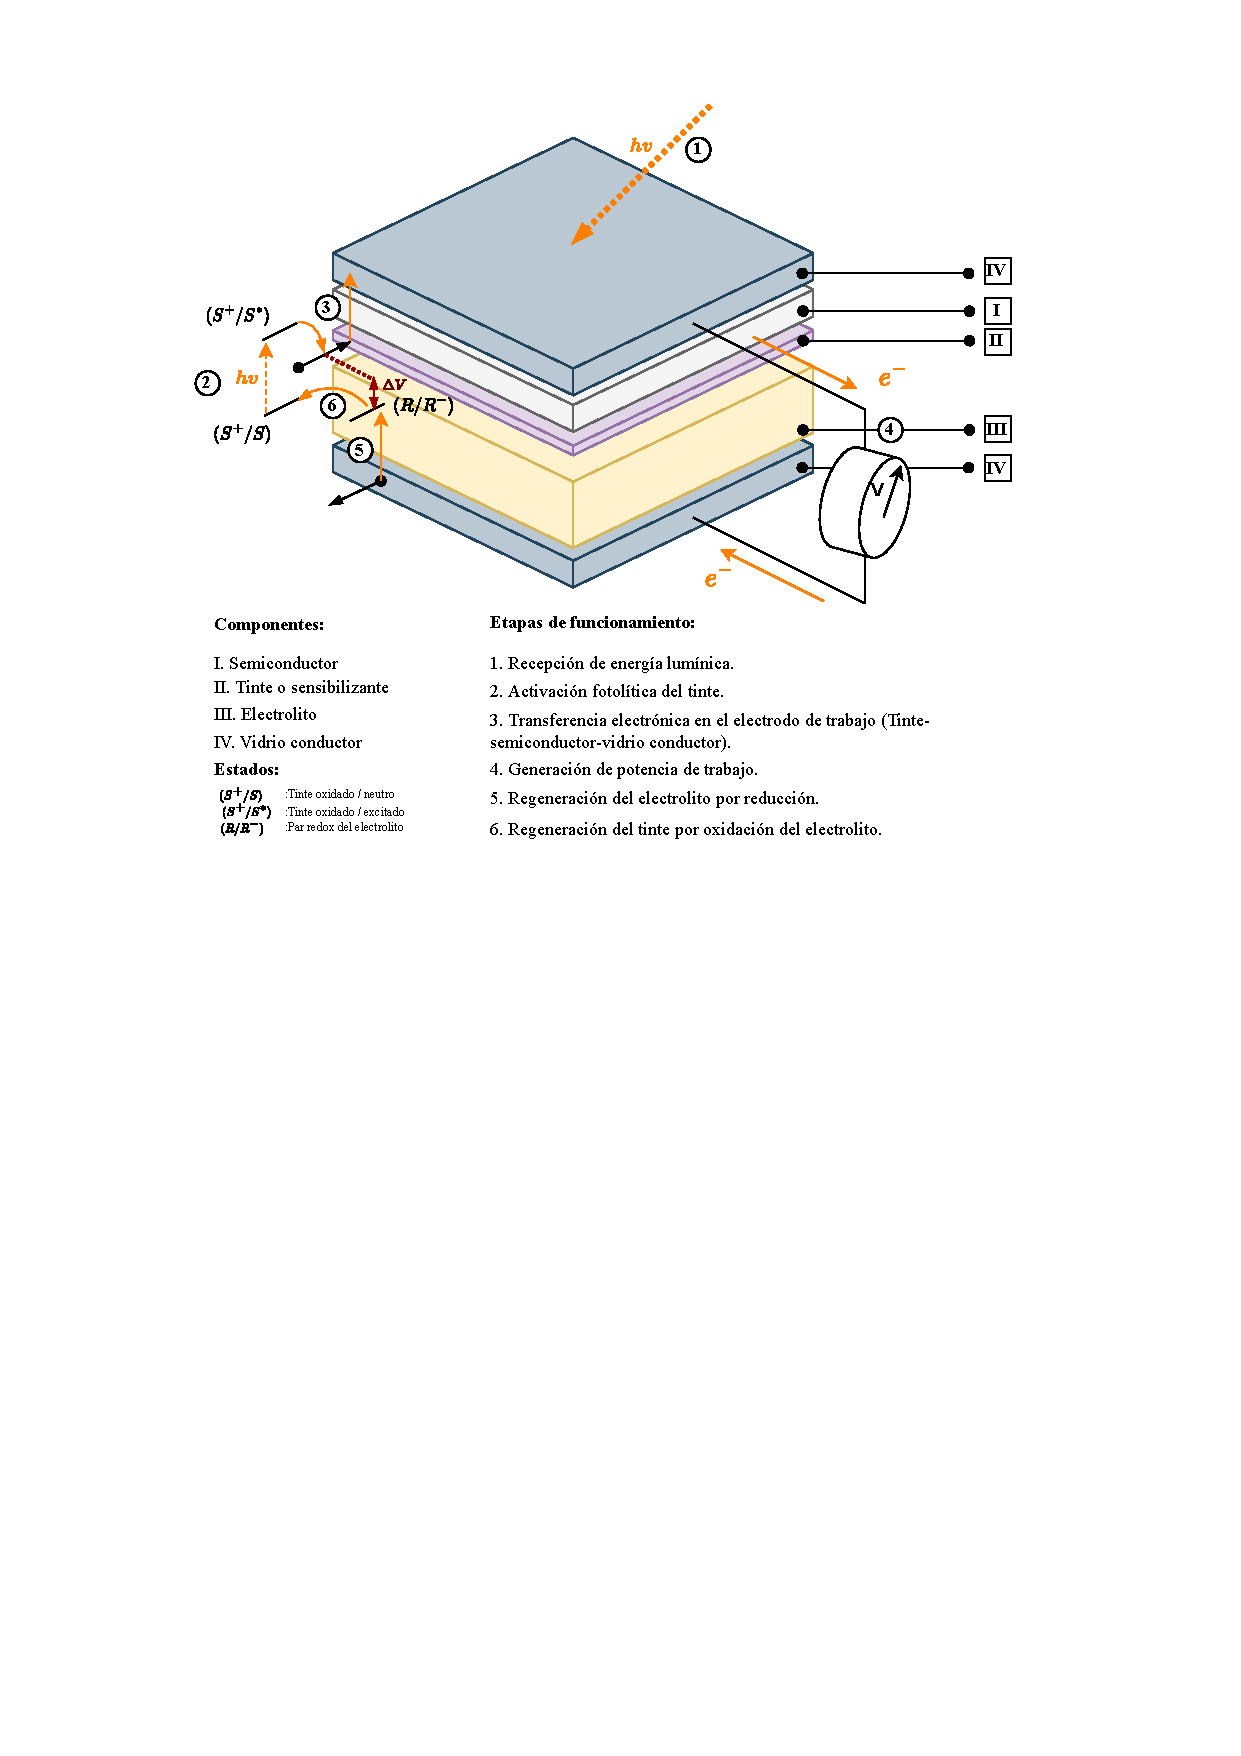
\includegraphics[clip, trim=0.5cm 14cm 0.5cm 1cm, width=1.00\textwidth]{img/diagrama_tesis.pdf}
        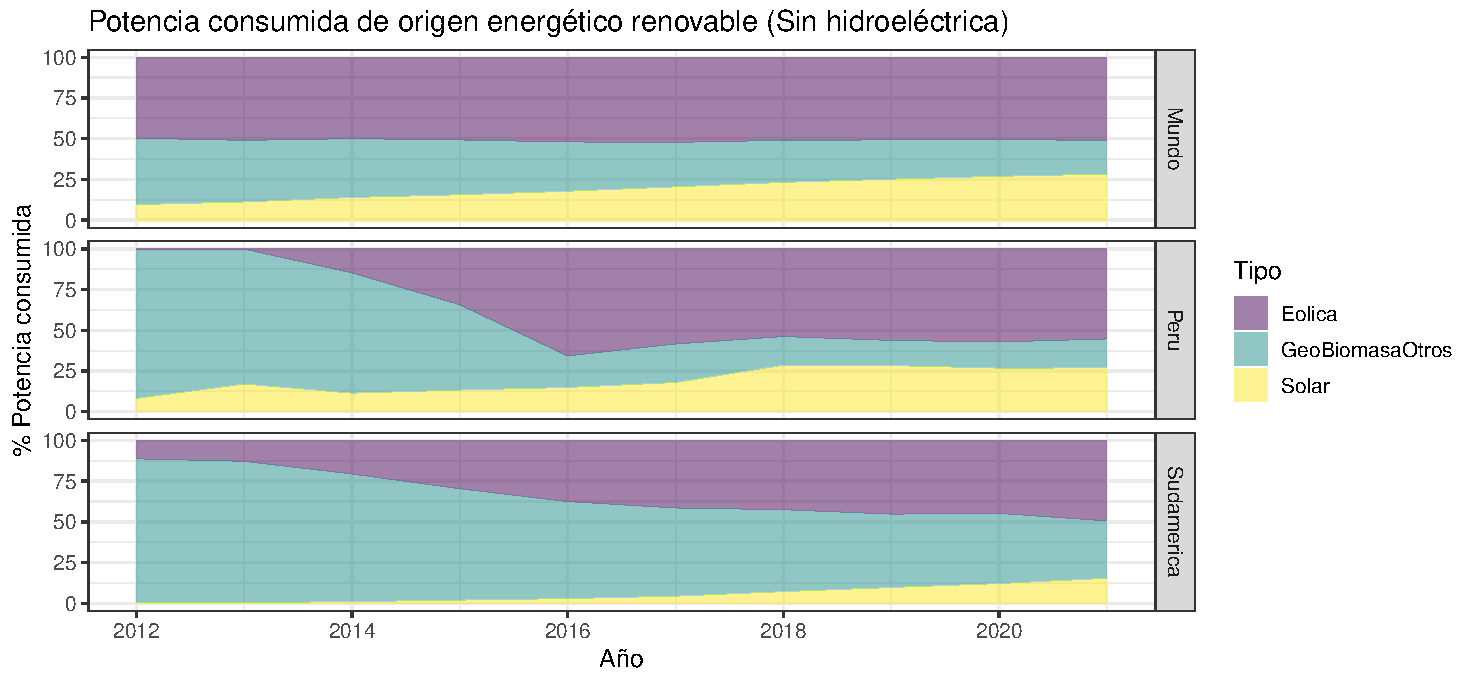
\includegraphics[scale=0.7]{img/renovables.pdf}
    \end{center}
    \caption{Comparación del porcentaje de la cantidad de potencia consumida por tipo de energía renovable sin considerar la hidroeléctrica.
    Fuente: Our World in Data \cite{owidenergy}}
    \label{img:PorcentajeRenovable}
\end{figure}

Hace un año, la energía hidroeléctrica generó más de 4 mil tera-vatios por hora (TWh) en el mundo, lo que representó más del 50\% de la generación de todas las renovables \cite{irena2022international}. No obstante, no es posible extender la construcción de centrales hidroeléctricas dado que muchas comunidades no cuentan cuencas hidrográficas o caídas de agua que puedan aprovecharse. Sin contar esta fuente, las energías eólica y solar son las que encabezan la producción energética. Con el propósito de contextualizar el crecimiento del uso de estas fuentes renovables geográfica y temporalmente se muestra la Figura \ref{img:PorcentajeRenovable}. En ella se visualizan los porcentajes de potencia consumida provenientes de tres grupos de fuentes renovables no hídroeléctricas: La eólica, solar y otras (\textit{GeoBiomasaOtros}). Estos porcentajes se distribuyen desde el 2012 hasta el 2021 y se comparan las tendencias en el Perú, Sudamérica y el mundo. Se aprecia el aumento del consumo energético de la eólica y solar sobre las demás, y de entre estas dos, la eólica es mayor. No obstante, también es evidente que la energía solar ha tenido un crecimiento sostenido en el tiempo y esto se debe, entre otras razones, a la disponibilidad de nuevas tecnologías más comercial y ambientalmente más viables que aprovechan la luz solar.



Existen dos tipos de tecnlogías solares: La termosolar y la fotovoltaica \cite{hammarstrom2012}. En la primera se usa la energía térmica de un fluído calentado por concentradores solares para generar electricidad por medio del movimiento de turbinas contectadas a generadores electromagnéticos. Pese a los esfuerzos por reducir los costos de construcción y mantenimiento de las centrales termosolares, solo países con alta demanda energética industrial y la geografía apta pueden hacer rentables estas tecnologías \cite{xu2022concentrated}.


En contraste a la termosolar, en la fotovoltaica se aprovecha directamente la radiación solar mediante fenómenos fotoeléctricos y de transporte de cargas, mimetizando la fotosíntesis. Si las plantas tienen a las células con clorofila en sus hojas como sus unidades generadoras de energía, en los sistemas fotovoltaicos estas serían las células o celdas solares. La estructura de una celda solar depende de los mecanismos de generación eléctrica y trasporte de carga, y estos a su vez, de la naturaleza de los materiales donde suceden estos mecanismos. El interés por desarrollar tecnologías fotovoltaicas se da por dos razones: Por su versatilidad, es decir que pueden ser usadas para fines domésticos o industriales, y  porque reducirían notablemente las emisiones de \ce{CuO2}/kWh, por ejemplo esta reducción sería cercana al 90\% para sistemas que sustituyan al gas natural \cite{tawalbeh2021environmental}.


Las celdas solares llevan en el mercado más de 60 años, desde su descubrimiento en los  Laboratorios Bell en 1954 \cite{green2009path} y su primer uso comercial en el satélite Vanguard \cite{singh2013solar} en 1958, estos se han diversificado en su composición, por ende, también en su eficiencia y estabilidad. Según la clasificación del \textit{National Renewable Energy Labotatories} (NREL) los tipos de celdas se pueden agrupar en cinco familias: Cristalinas de silicio, de unión simple de galio (Ga) y arsénico (As), de unión múltiple, basadas en películas delgadas y emergentes \cite{nrel}. Los puntos en común de estas familias son la similitud de sus componentes, arquitecturas y/o coetaniedad \cite{blakers2013}. Cabe mencionar que en adelante solo se tomarán en cuenta tecnologías fotovoltaicas que no tengan concentradores.


En primer lugar se encuentra la familia de las celdas basadas en cristales de silicio que congrega a las celdas de monocristal \cite{gul2016}, multicristal\cite{moller2005multicrystalline}, con heteroestructuras de silicio \cite{sark2012introduction} y con películas delgadas de silicio cristalino \cite{brendel2011thin}. Segundo, las celdas de unión simple (Ga-As) en donde están las que se basan en cristales y las de películas delgadas \cite{konagai1978high}. Tercero, las celdas de unión múltiple que tienen celdas con arquitecturas con dos, tres y cuatro a más uniones \cite{dimroth2007high, philipps2018high}. Cuarto, en las celdas basadas en películas delgadas están las celdas de cobre-indio-galio-selenio (CIGS) \cite{wada2001high}, cadmio-teluro (CdTe) \cite{ferekides2004cdte} y silicio amorfo hidrogenado (a-Si:H) \cite{krvc2003analysis}. Y en quinto lugar, las celdas emergentes, que se caracteriza por agrupar las tecnologías que llevan menos tiempo siendo investigadas tales como las celdas sensibilizadas por tintes (CSPT) \cite{sharma2018dye}, las inorgánicas basadas en kesterita \ce{Cu2ZnSn(S,Se)4} (CZTSSe) \cite{suryawanshi2013czts}, las celdas orgánicas \cite{hoppe2004organic}, orgánicas tipo \textit{sándwich} \cite{ameri2009organic}, las celdas perovskitas \cite{jung2015perovskite}, perovskitas-CIGS monolítica tipo \textit{sándwich} \cite{li2020perovskite}, perovskitas-SI monolítica tipo \textit{sándwich} \cite{li2020perovskite} y celdas con \textit{quantum-dots} \cite{kim2022conformal}. 

\begin{figure}[h!]
    \begin{center}
        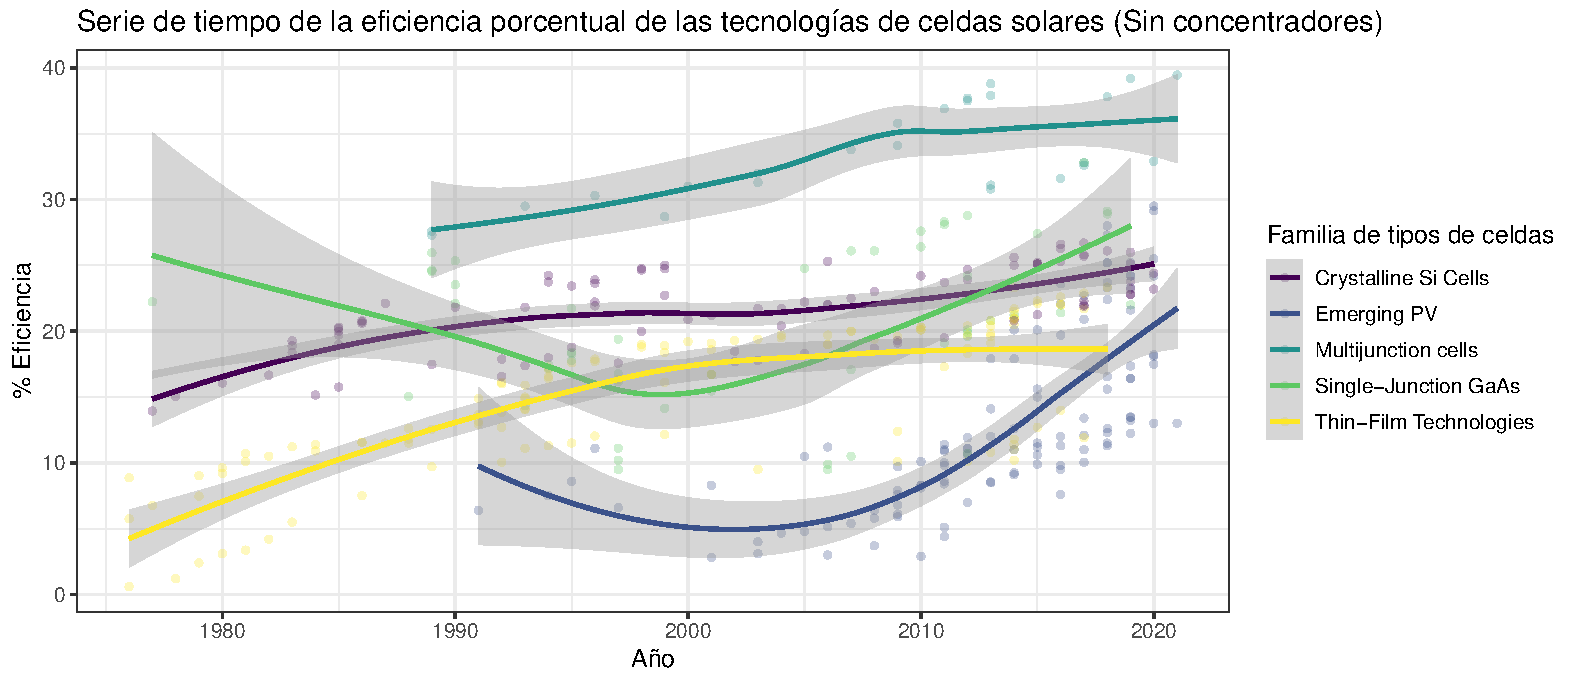
\includegraphics[scale=0.6]{img/familia_celdas.pdf}
    \end{center}
    \caption{Serie de tiempo de las mejores eficiencias obtenidas en la investigación de las celdas solares según la agrupación dada por NREL.
    Fuente: \textit{National Renewable Energy Laboratory} \cite{nrel}}
    \label{img:SerieTiempo}
\end{figure}

Para contrastar dichas tecnlogías se pueden usar las mejores eficiencias de conversión energética de estos dispositivos obtenidos en el laboratorio que fueron recopilados por la NREL entre los años de 1980 y 2021 (Figura \ref{img:SerieTiempo}). En esa gráfica se observa que las tecnologías con mayor rendimiento han sido las celdas de unión múltiple, esto se debe a que sus arquitecturas fueron diseñadas para que haya un efecto sinérgico gracias a la apilación de los mejores materiales fotoeléctricos y de transporte de carga que existían en su época, no obstante, estos serían más costosos que los demás por la mayor cantidad y diversidad de materiales que se demandan para fabricarlos. También se aprecia que las tendencias de investigación de las celdas de silicio cristalino y las películas delgadas han desacelerado el aumento de sus rendimientos a diferencia de las celdas de unión simple Ga-As o emergentes. Es probable que esto sea consecuencia del descubrimiento de nuevos materiales con menores costos de producción, ambiental y con buen desempeño, por ejemplo: Moléculas orgánicas aceptoras-donadoras o \textit{quantum dots}.


Es un hecho que las tecnlogías emergentes están igualando, en términos de performance en el laboratorio, a las celdas comercialmente más comúnes como lo son las que se silicio multicristalino y las películas de Ga-As \cite{chowdhury2020overview}. Es por ello que es importante seguir investigándolas, pero como se mencionó anteriormente, esta familia reune diversas tecnologías y por tal motivo es importante sopesarlas desde el punto de vista de la sostenibilidad.

Con los datos del NREL se construyó una serie de tiempo de las mejores eficiencias que muestran en el laboratorio todos los tipos de celdas que pertenecen a las tecnologías emergentes  (Figura \ref{img:SerieEmergente}). En dicha gráfica se da cuenta que las celdas basadas en perovskitas encabezan a las demás y a su vez son las más recientes en ser exploradas, este material está compuesto por átomos de titanio y calcio dispuestos ortorrómbicamente cuando es cristalino, tiene un \textit{bandgap} de 1.5 eV, un alta constante dieléctrica, capacidad de separar rápidamente la carga y de ser funcionalizados con CIGS, Si, Sn y/o Pb para extender el rango de absorción del expectro solar (300-800 nm) y aumentar el coeficiente de absorción ($10^5cm^{-1}$) \cite{velilla2019outdoor}. A pesar de que estas ventajas han hecho de las celdas de perovskitas las más promisorias de las emergentes, la exposición al ambiente de estos dispositivos serían tóxico para la salud de los seres vivos, debido al Sn o Pb \cite{wang2022sustainable}. Otras celdas que presentan el mismo problema son las que tienen \textit{quantum dots}\cite{pan2014high} o compuestos inorgánicos CZTSSe\cite{suryawanshi2013czts}, ya contienen Cd y Sn respectivamente, aparte que hay esfuerzos por mejorar su estabilidad y disminuir sus costos de fabricación, los cuales dificultan su comercialización. 

Contrario a las ya mencionadas tecnologías emergentes, las celdas orgánicas y las celdas sensibilizadas por tintes (CSPT) son más sostenibles gracias a la capacidad de degradación de los polímeros que los componen, además tienen otras ventajas como lo son su construcción por módulos o etapas, las diversas estructuras químicas de sus componentes orgánicos o metal-orgánicas y, en consecuencia, costos de fabricación accesibles de ser escalados para fines comerciales. Si bien las CSPT han sido las primeras en ser investigadas, las celdas orgánicas las han superado en términos de eficiencia debido al descubrimiento de materiales compuestos por moléculas aceptoras y donadoras de alto rendimiento para generar y transportar carga \cite{li2022recent}. Estos descubrimientos fueron guiados por conocimiento específico de las relaciones que hay entre la estructura y las propiedades de las moléculas, en la etapa de diseño y posteriormente evaluadas experimentalmente. No obstante, aún hay brechas en el conocimiento de la existencia de tintes que sean capáces de equiparar a sus similares orgánicas. Complementando la anterior idea, existe la probabilidad de encontrar tintes con propiedades de interés fotovoltaico extraídos de la biodiversidad peruana, lugar donde se realizará el presente proyecto.

\begin{figure}[h!]
    \begin{center}
        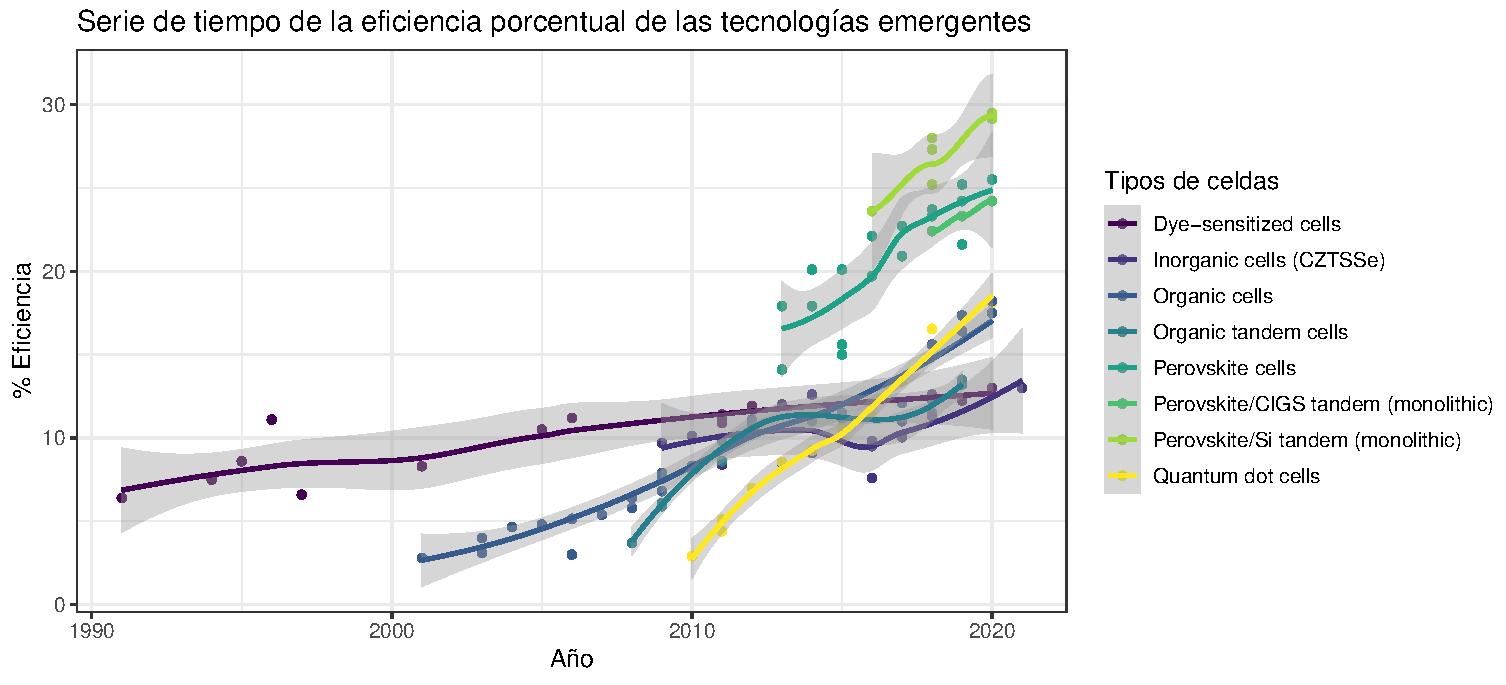
\includegraphics[scale=0.6]{img/emergentes.pdf}
    \end{center}
    \caption{Serie de tiempo de las mejores eficiencias obtenidas en la investigación de las tecnologías emergentes de celdas solares.
    Fuente: \textit{National Renewable Energy Laboratory} \cite{nrel}}
    \label{img:SerieEmergente}
\end{figure}

Entiéndase por tintes o colorantes a las sustancias que estén constituídas por una mezcla de varias moléculas dentro de una fase líquida o sólida que muestran una coloración dentro de un rango de longitudes de onda. Mientras que las CSPT son dispositivos que aprovechan sus propiedades fotoactivas dentro de uno de sus componentes. Las arquitecturas de las CSPT se componen por 4 materiales: El semiconductor, el tinte o sensibilizador, el electrolito y los vidrios conductores (Figura \ref{img:CSPT}). Las CSPT modernas derivan de la celda creada por Brian O'Rigan y Michael Gratzel en 1991 \cite{o1991low}, la cual comúnmente se usa para exponer el funcionamiento de estos dispositivos. En dicha celda, se usó óxido de estaño dopado con flúor y partículas de platino (Pt-FTO) como vidrio conductor, el cuál soportaba el óxido de titanio \ce{TiO2} nanocristalino dopado a su vez por nanopartículas de complejos triméricos de rutenio(II) bipidirina (Rutenio-bipidirina) como semiconductor y tinte sensibilizante, respectivamente. Para la regeneración del tinte se utilizó yoduro/triyoduro como electrolito redox. El fotovoltage ($\Delta V$) de celda corresponde al potencial teórico de trabajo útil y puede aproximarse a la diferencia entre el nivel de energía de Fermi del semiconductor bajo iluminación y el potencial de Nernst del par redox del electrolito.

\begin{figure}[!thb]
    \begin{center}
        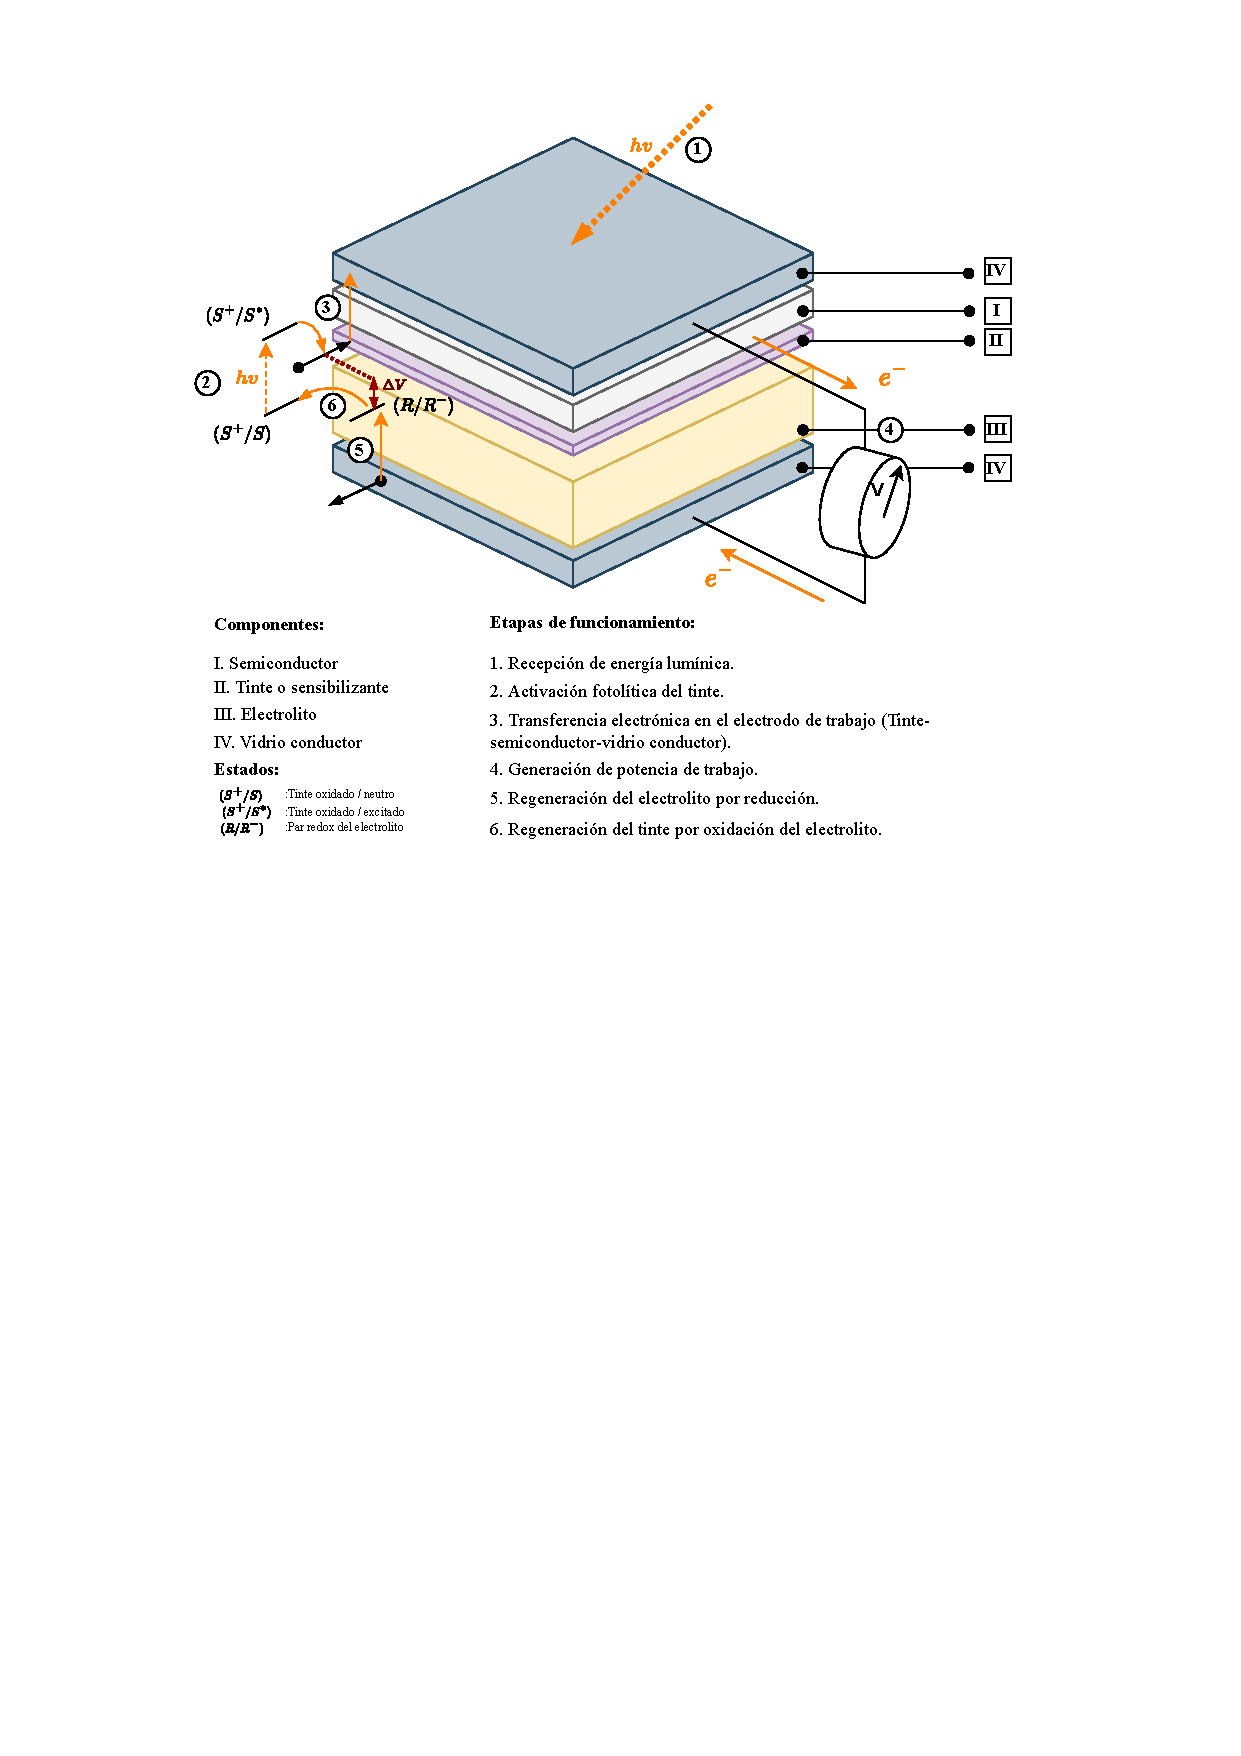
\includegraphics[clip, trim=0.5cm 14cm 0.5cm 1cm, width=1.00\textwidth]{img/diagrama_tesis.pdf}
    \end{center}
    \caption{Estructura y funcionamiento de una celda solar sensibilizada por tinte (CSPT). Fuente: \textit{O'Rigan y Grätzel} \cite{o1991low}}
    \label{img:CSPT}
\end{figure}


Cada uno de los componentes influyen directamente al rendimiento de la celda en términos de dos ecuaciones: La eficiencia de corriente monocromática ($\eta_{i} (\lambda)$) y la eficiencia del potencial de conversión (PCE). La  ecuación \ref{eqn:nil} describe la capacidad del dispositivo para mantener el flujo eléctrico de celda generado por fenómenos fotoeléctricos. Esta capacidad se calcula como el producto de la eficiencia de recolección de luz de longitud $\lambda$ ($\text{LHE}(\lambda)$) que mide la fracción de fotones incidentes que son absorbidos por el tinte, el rendimiento cuántico de inyección de carga ($\phi_{inj}$) que mide el número de huecos inyectados hacia la capa de valencia o electrones a la banda de conducción del semiconductor sensibilizado por número de einstein absorbidos, y la eficiencia de colección de carga de retorno ($\eta_e$) que mide la fracción de electrones que llegan al contraelectrodo versus los que salieron del electrodo de trabajo en un circuito cerrado. Como esta medición sólo toma en cuenta valores de parámetros para una longitud de onda, es más práctico tomar como medida de referencia la segunda ecuación.


\begin{equation}
    \eta_{i}(\lambda) = \text{LHE}(\lambda)\times \phi_{inj} \times \eta_e
    \label{eqn:nil}
\end{equation}

Por otra parte, la  ecuación \ref{eqn:pce} describe a la eficiencia del potencial de conversión como el porcentaje del potencial lumínico del haz incidente aprovechado en forma de potencial eléctrico de salida. Para calcularlo, la CSPT es sometida a mediciones de densidad de corriente y voltage ($J/V$) en presencia de luz de un simulador solar. Los parámetros extraídos de estos experimentos son la densidad de corriente de corto circuito ($J_{SC}$), el voltaje del circuito abierto ($V_{OC}$), el factor de llenado ($FF$) y la potencia incidente ($P_{in}$). El $J_{SC}$ permite conocer las características de absorción de la capa fotoactiva, la generación y el transporte de carga; debido a que estas la afectan. Mientras que el $V_{OC}$ permite obtener la información de los niveles de energía de los materiales fotoactivos, el estado del funcionamiento de los materiales del electrodo de trabajo y la velocidad de recombinación del portador de carga. Por la parte del $FF$, que se define como la relación entre la potencia real de la celda y la potencia sin la presencia de resistencia; es posible colectar información del estado de los electrodos y la estabilidad de los materiales en un determinado tiempo. Cabe señalar que el $FF$ idealmente debe ser 1, lo cual signfica que no existen fenómenos de desgaste que consuman potencial de trabajo. \underline{Añadir Referencias}

\begin{equation}
    \text{PCE} = \frac{P_{out}}{P_{in}}  =\frac{J_{SC}\times V_{OC} \times FF}{P_{in}} \times 100\%
    \label{eqn:pce}
\end{equation}

Teniendo en cuenta las formas de medir el desempeño de una celda solar, es evidente que el reto de mejorar estos dispositivos recaiga en gran parte en los materiales con los que son hechos. En especial por los tintes que son los responsables de 

\begin{figure}[h!]
    \begin{center}
        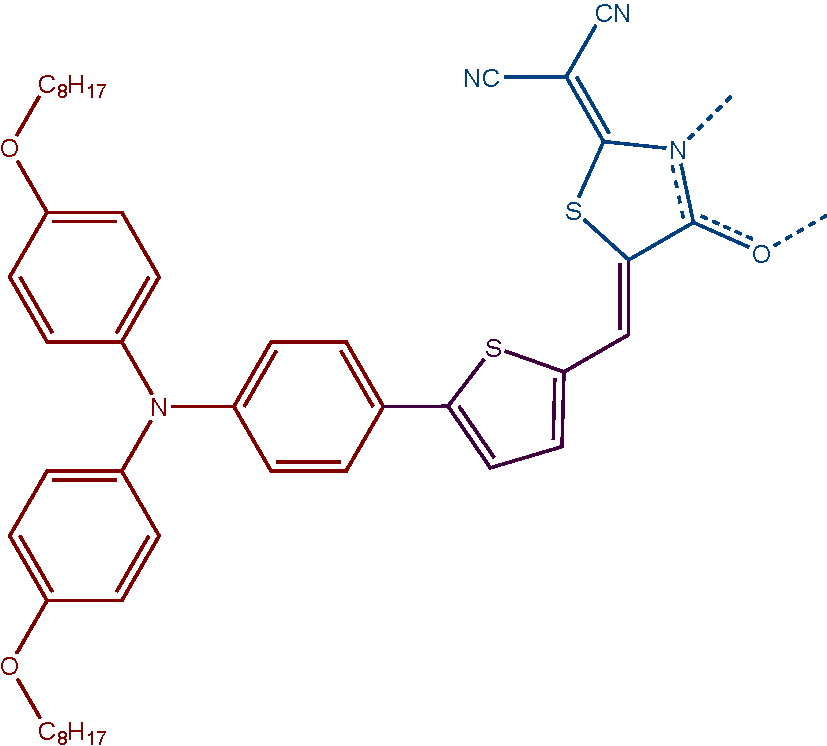
\includegraphics[scale=0.5]{img/dye_scheme.pdf}
    \end{center}
    \caption{Esquema de un tinte Fuente: https://doi.org/10.1002/anie.201204948}
    \label{img:tinte}
\end{figure}


Los efectos fotovoltaicos suceden cuando los fotones caen sobre un semiconductor que produce pares de electrones-hoyo que suceden en la interfaz entre dos materiales diferentes. Este fenómeno es el que crea el diferencial de potencial.

Las celdas inorgánicas y electroquímicas operan cuando se establece un diferencial de potencial entre dos materiales con propiedades electrónicas diferentes (tipo n y p) o entre los semiconductores n o p y un electrolito redox. 


Como regla general, fotones con energía igual al $E_g$ de un material será absorbido generando electrones libres, mientras que si es menos pasará através de este él o si es mayor convertirá el exceso de energía en calor. (Barttalota)


%%%%%%%%%%%%%%%%%%%%%% ADICIONAL DE VENTAJAS DE CSPT  %%%%%%%%%%%%%%%%%%%%%% 

Las CSPT aplican mecanismos diferentes a los otros dispositivos fotovoltaicos. En contraste a los sistemas convecionales que utilizan semiconductores donde en este suceden los mecanismos de absorción de luz y el transporte de carga, los CSPT tienen estos dos mecanismos separados. En las CSPT el tinte sensibilizante se ancla al semiconductor absorbe la luz, mientras que la separación de carga se da en el interfaz del sensibilizante y la banda de conducción del semiconductor por medio de inyección fotoinducida de electrones. Estas características les confieren a las CSPT las ventajas de ser diseñadas e implementadas modularmente así como de operar establemente, incluso en condiciones de temperatura, irradiación y ángulo de incidencia solar no estándares. Adicionalmente, la construcción de las CSPT no requiere altas temperaturas o sistemas de vacío. Gracias a las ventajas de las CSPT, existen esfuerzos para mejorar sus propiedades así como darle usos comerciales. Un ejemplo de esto último son los primeros CSPT comerciales usados como sensores y electrónica domótica ofrecidos en el 2009 por la empresa israelí 3G Solar Photovoltaics Ltd.  (https://www.3gsolar.com/.)


%%%%%%%%%%%%%%%%%%%%%% FUNCIONAMIENTO DE LAS CSPT  %%%%%%%%%%%%%%%%%%%%%% 

El electrolito puede ser líquido, gel o sólido y se une al semiconductor como fase de contacto, las otras celdas se unen por contacto de fases sólidas. 
El corazón del sistema Grätzel es el fotoánodo que consiste en una monocapa de tinte sensibilizante absorbido por una capa de un semiconductor mesoporoso, de aproximadamente 10 $\mu$ m de grosor. El semiconductor usualmente es \ce{TiO2}, pero también puede ser \ce{ZnO,SnO2, Nb2O5}, etc. El electrolito que permeabiliza el semiconductor y que dona electrones a las moléculas oxidades del tinte es comúnmente el par redox yoduro/yodo.
Bajo la radiación lumínica el tinte promueve electrones (\ce{e^-}) del HOMO al LUMO. El LUMO debe tener mayor energía que la banda de conducción el semiconductor para que la inyección suceda, posteriormente los electrones excitados difunden por el semiconductor y son colectados por el óxido conductor del vidrio FTO/ITO. Estos electrones salen del fotoánodo hacia el cátodo y en su paso pueden ser aprovechados como potencial eléctrico (\textit{V}). Al reentrar a la celda por medio del contra electrodo (típicamente a construído a base de Pt-s/TCO), los electrones reducen los transportadores de huecos de electrones (\ce{I3^- -> I^-}). Por último el agente reductor del electrolito difunde hacia el semiconductor pra regenerar el tinte oxidado en cuestión de micro segundos, de tal forma que cierre el ciclo operativo de óxido-reducción de la celda sin afectar teóricamente las estructuras químicas de los componentes.

%%%%%%%%%%%%%%%%%%%%%% OPTIMIZACIÓN DE LAS CSPT  %%%%%%%%%%%%%%%%%%%%%% 

No obstante, existen reacciones que merman el rendimiento, las cuales son: El decaimiento del estado excitado del tinte, la migración de electroles de la banda conductora del semiconductor al tinte o al electrolito, también conocidas como reacciones de retroceso y oscuras, respectivamente. 

Teniendo en cuenta lo anterior, se infiere que la optimización de las celdas CSPT recae en contrarrestar al máximo dichas reacciones. Una manera de hacerlo es diseñando rutas para que la inyección electrónica y la regeneración del tinte por medio del electrolita sean más rápidas que el decaimiento del tinte excitado y las reacciones de retroceso, respectivamente. 

%%%%%% Falta completar la optimización 
Es claro que deben de validarse experimentalmente los resultados obtenidos por los métodos computacionales, pero estos pueden discriminar cientos de candidat


%%%%%%%%%%%%%%%%%%%%% SOBRE LOS TINTES NATURALES %%%%%%%%%%%%%%%%%%%%%%%%

Los tintes sensibilizantes ideales deben absorber un amplio rango de longitudes de onda, en especial cubrir la región visible y cercana al infrarrojo. Además de mostrar alta foto estabilidad, una absortividad molar grande y debe ser capaz de inyectar los electrones fotogenerados rápidamente desde su estado excitado a la banda de conducción del semiconductor. Esto se logra con un fuerte anclaje a la superficie del óxido conductor y con un potencial redox propicio que permita su rápida regeneración gracias al electrolito. No obstante, las celdas tienen un tiempo de vida a causa de los procesos de enfriamiento o \textit{quenching} y otros generados por el medio que degradan al tinte o al electrolito.

(G. Calogero, A. Bartolotta, G. Di Marco, A. Di Carlo, F. Bonaccorso, Vegetablebased
dye sensitized solar cells, Chem. Soc. Rev. 44 (2015) 3244e3294.)

Hasta la fecha se han clasificado los tintes sensibilizantes en tres clases: Basados en complejos metálicos, en estructuras orgánicas libres de metales y de fuentes naturales.

Aquellos basados en complejos metálicos tienen dos tipos de ligantes: De anclaje y auxiliares. Los ligantes de anclaje son responsables de absorber el tinte a la superficie del semiconductor. Por otro lado, los ligantes auxiliares permiten la modulación de las propiedades del complejo. Algunos tintes de este tipo son los derivados del bipiridil de rutenio como el N3, N719 y el N749 o tinte negro. A pesar que estos tintes tienen altas eficiencia de conversión ($\eta$), sus altos costos de fabricación, limitados coeficientes de extinción y potenciales efectos contaminantes derivados de los metales dificultan la sostenibilidad de las CSTP y por ende la investigación basada en estos materiales.

En segundo lugar, los tintes orgánicos libre de metales resuelven las limitaciones anteriormente mencionadas, ya que pueden ser diseñadas molecularmente para que estos presenten altos coeficientes de extinción molar y estabilidad bajo condiciones no estándares de temperatura y iluminosidad. Generalmente, las estructuras de estos tintes se configuran químicamente en regiones donadoras y aceptoras de electrones, y puentes conjugados que unen y espacian dichas regiones ($D-\pi-A$). Las configuraciones donadoras de electrones pueden ser cumarinas, fenilaminas, indolinas, triarilaminas, carbazoles, entre otras. Mientras que las estructuras aceptoras pueden ser ácido cianoacrílico, rodaminas o piridinas. Por otra parte las configuraciones puentes pueden ser derivados de tiofenos, polienos o benzotiadiazoles. 

Por último, la clase de tintes naturales son aquellos que se extraen de seres vivos, mayoritariamente de fuentes vegetales como frutas, flores, hojas, entre otras. Muchos de los pigmentos vegetales extraídos han sido investigados como sensibilizantes para CSTP y presentaron rendimientos fotovoltaicos significativos, en especial colorantes como derivados de clorofila, betalaínas, antocianicas, carotenoides, etc. 


pero dado un grado de precisión razonable  en la predicción de la propiedad del material, estos modelos computcionales aceleran el proceso de elegir mejores estructuras o moléculas candidatas con la correcta combinación de propiedades necesarias para cumplir satisfactoriamente con el propósito para las que fueron hechas \textit{Leon R. Devereux}. 

\begin{figure}[h!]
    \begin{center}
        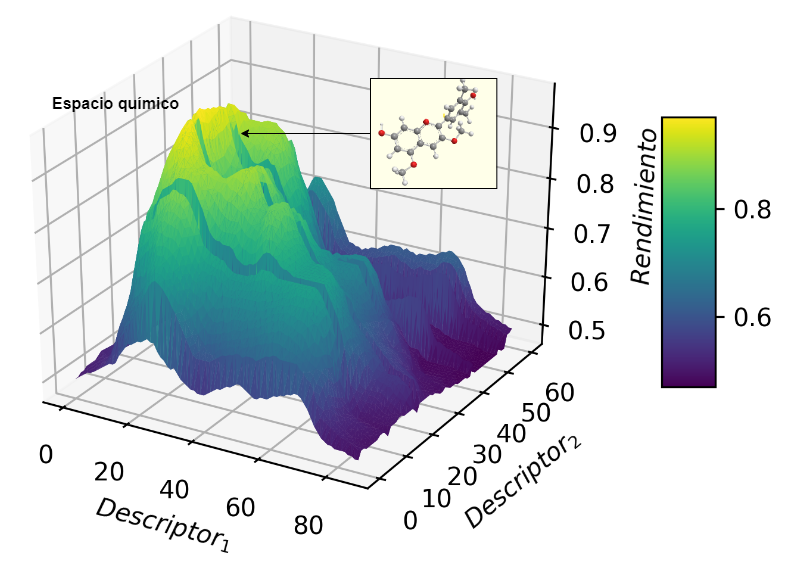
\includegraphics[scale=0.45]{img/espacioquimico.png}
    \end{center}
    \label{img:espacioquimico}
    \caption{Serie de tiempo de las mejores eficiencias obtenidas en la investigación de las celdas solares según la agrupación dada por NREL.
    Fuente: \textit{National Renewable Energy Laboratory} \cite{owidenergy}}
\end{figure}

\begin{figure}[h!]
    \begin{center}
        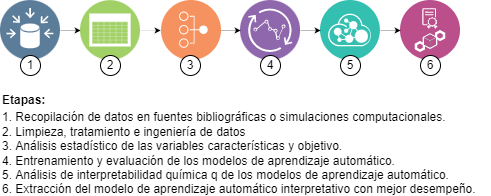
\includegraphics[scale=0.7]{img/etapas.png}
    \end{center}
    \label{img:etapas}
    \caption{Serie de tiempo de las mejores eficiencias obtenidas en la investigación de las celdas solares según la agrupación dada por NREL.
    Fuente: \textit{National Renewable Energy Laboratory} \cite{owidenergy}}
\end{figure}
